\chapter{Проектирование полосковых устройств и согласование компонентов.} \label{chap:parts_design}

\section{Проектирование МШУ}

Создадим схему усилителя. Для моделирования усилителя будем использовать блоки DAC и Amplifier2. Для размещения компонента на плате необходимо спроектировать и смоделировать посадочное место. На Рис~\ref{fig:PMA-Place} показаны обозначения элементов. Размеры приведены в таблице~\ref{tab:PMA-Place}

\begin{figure}[!ht]
	\centering
	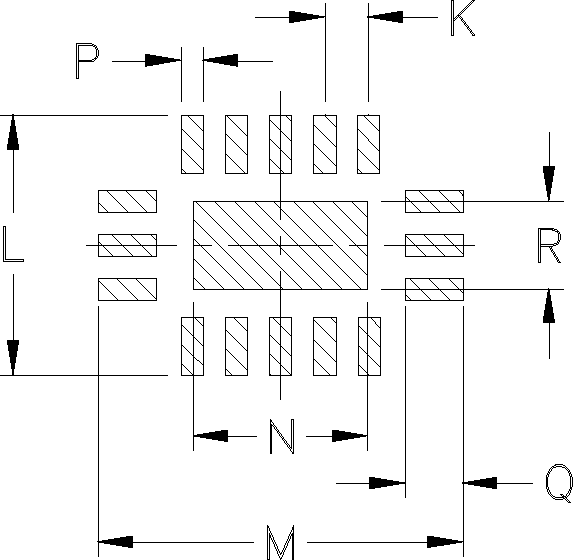
\includegraphics[width=0.45\textwidth]{PMA-Place.pdf}
	\caption{Рекомендуемое посадочное место.}%
	\label{fig:PMA-Place}
\end{figure}

\begin{table}[!ht]
	\renewcommand{\arraystretch}{1.5}
	\begin{center}
		\caption{Размеры падов, мм}\label{tab:PMA-Place}
		\begin{tabularx}{0.45\textwidth}{!{\vrule width 2pt}*{3}{>{\centering\arraybackslash}X|}>{\centering\arraybackslash}X!{\vrule width 2pt}}
			\bhline{2}
			P&K&\multicolumn{2}{|c!{\vrule width 2pt}}{Q} \\ \hline
			0.25&0.51&\multicolumn{2}{|c!{\vrule width 2pt}}{0.41} \\ \bhline{2}
			L&M&R&N \\ \hline
			3&4.19&1&2 \\ \bhline{2}
		\end{tabularx}	
	\end{center}
\end{table}

Вследствие изменения линии КСВН (равно как и другие характеристики) в рабочей полосе окажется испорченным. Для исправления этого недоразумения поставим входные и выходные согласующие цепи. Итоговые вид и параметры схемы можно увидеть на Рис~\ref{fig:LNA-Sch} и в Таблице~\ref{tab:LNA-Sch}. 

\begin{figure}[!ht]
	\centering
	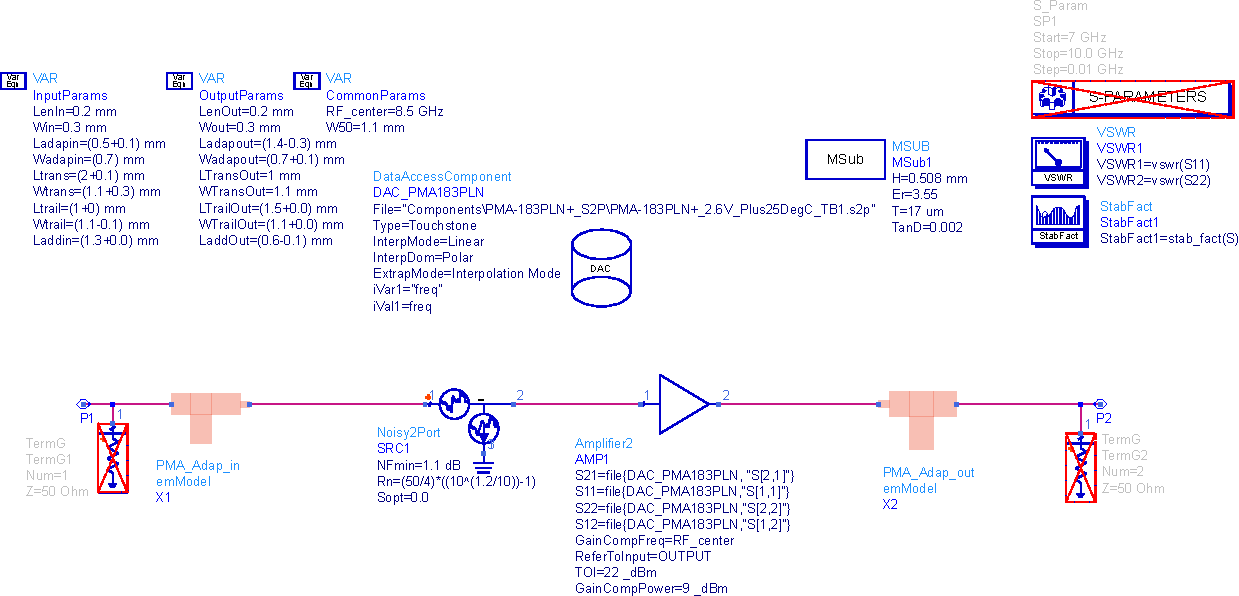
\includegraphics[width=0.95\textwidth]{LNA_Sch.pdf}
	\caption{Схема включения МШУ}%
	\label{fig:LNA-Sch}
\end{figure}

\begin{table}[!ht]
	\renewcommand{\arraystretch}{2}
	\begin{center}
		\caption{Параметры схемы}\label{tab:LNA-Sch}
		\begin{tabularx}{0.9\textwidth}{!{\vrule width 2pt}*{3}{>{\centering\arraybackslash}X!{\vrule width 2pt}}}
			\bhline{2}
			Параметр & Вход & Выход \\ \bhline{2}
			Подводная линия & Д=0.5 мм Ш=0.3 мм & Д=0.5 мм Ш=0.3 мм \\ \hline
			Трансформаторная линия & Д=1.5 мм Ш=1.1 мм & Д=0.9 мм Ш=1.1 мм \\ \hline
			Шлейф & Д=1.5 мм Ш=1.1 & мм Д=1.5 мм Ш=1.1 мм \\ \hline
			Наружная выводная линия & Д=1.0 мм Ш=1.1 мм & Д=1 мм Ш=1.1 мм
			\\ \bhline{2}
		\end{tabularx}	
	\end{center}
\end{table}

Результат согласования можно увидеть на Рис~\ref{fig:LNA-data}

\begin{figure}[H]
	\captionsetup{singlelinecheck=off, justification=centering}
	\centering
	\begin{subfigure}[b]{0.45\textwidth}
		\centering
		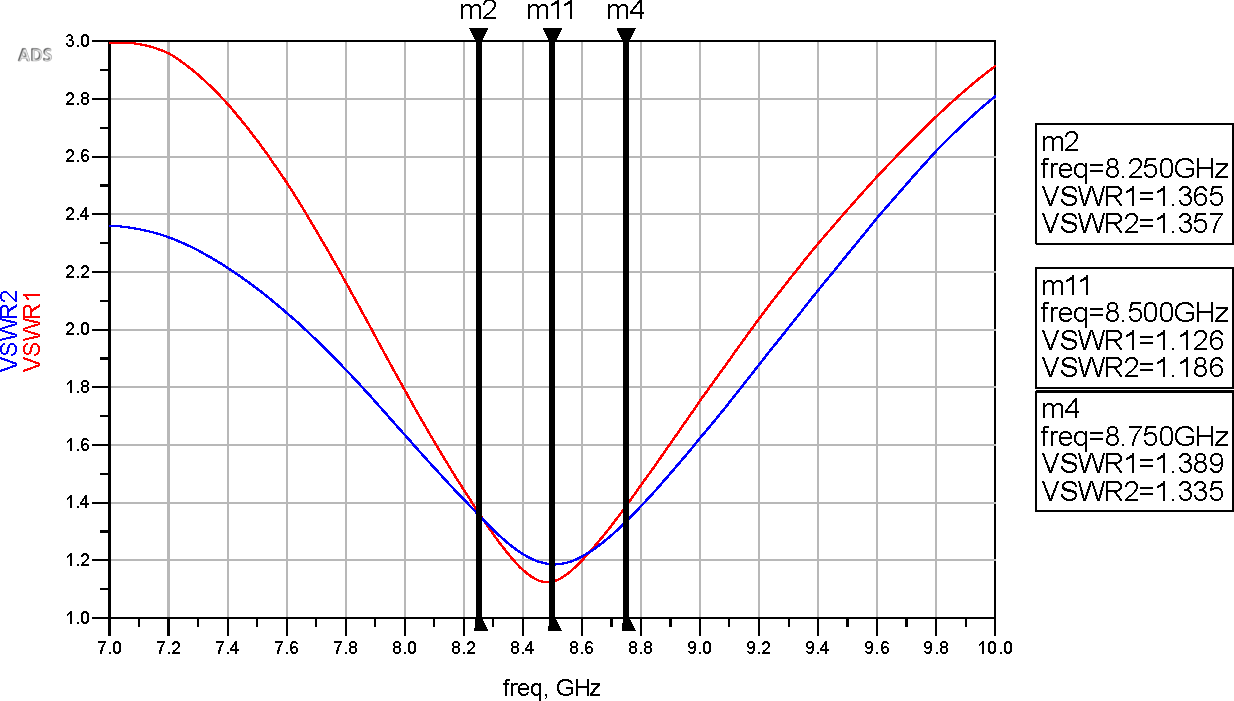
\includegraphics[width=\textwidth]{LNA_VSWR.pdf}
		\caption{}%
		\label{fig:LNA_VSWR}
	\end{subfigure}
	\hfill
	\begin{subfigure}[b]{0.45\textwidth}
		\centering
		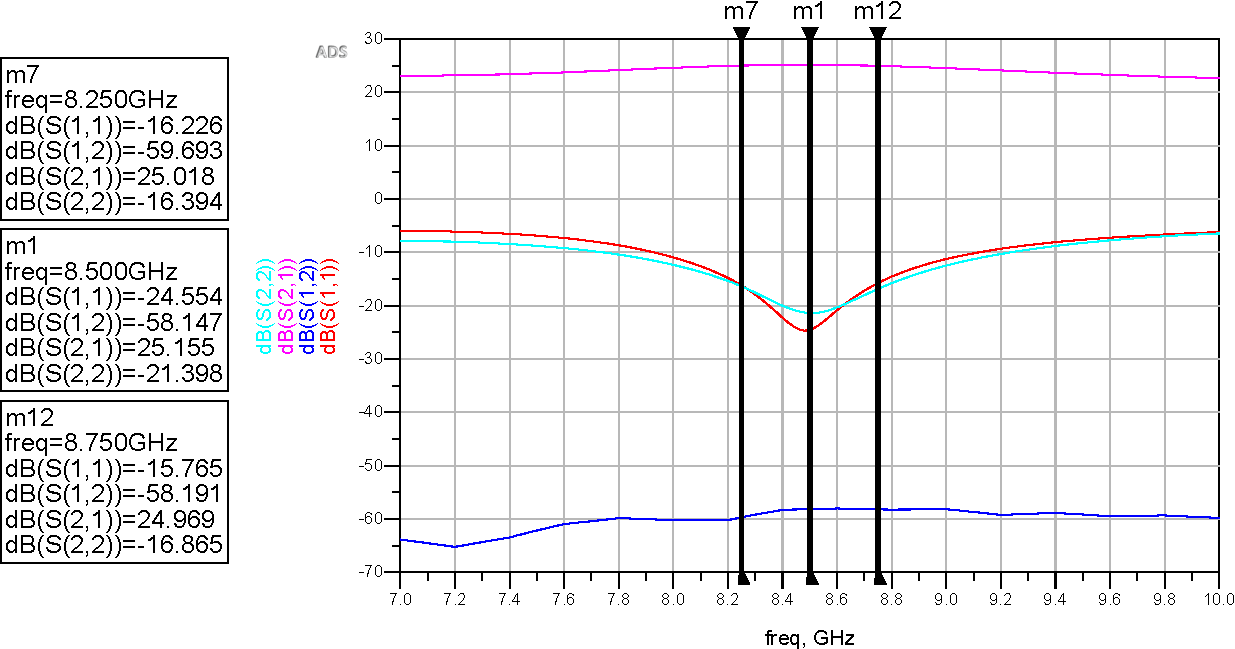
\includegraphics[width=\textwidth]{LNA_Response.pdf}
		\caption{}%
		\label{fig:LNA_Response}
	\end{subfigure}
	\hfill
	\begin{subfigure}[b]{0.9\textwidth}
		\centering
		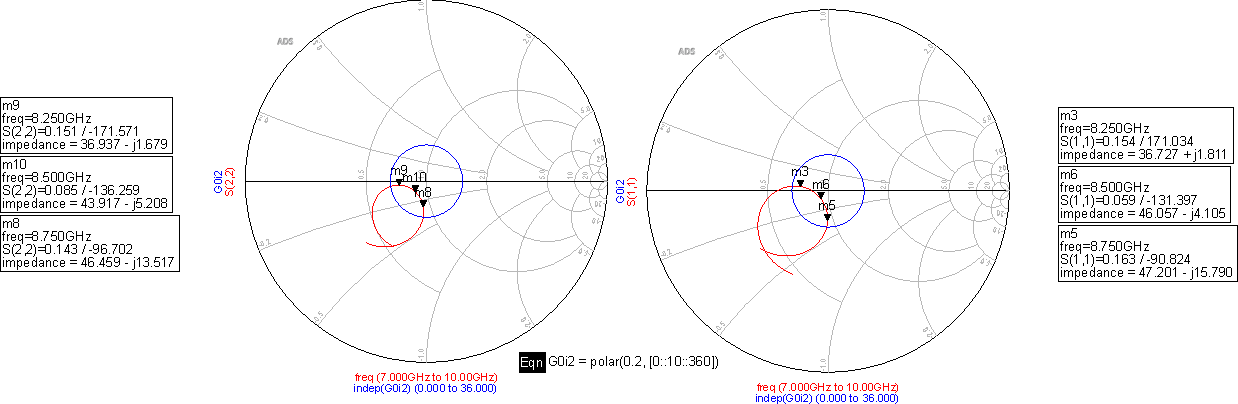
\includegraphics[width=\textwidth]{LNA_Response_Z.pdf}
		\caption{}%
		\label{fig:LNA_Response_Z}
	\end{subfigure}
	
	\caption{%
		Частотные характеристики проектируемого усилителя:
		(а) КСВН;
		(б) АЧХ;
		(в) Входное и выходное сопротивление
	}%
	\label{fig:LNA-data}
\end{figure}

\section{Посадочное место детектора мощности}

Для моделирования схемы включения детектора мощности будем использовать блок S1P. Для размещения компонента на плате необходимо спроектировать и смоделировать посадочное место. На Рис~\ref{fig:LTC-Place} показаны размеры элементов. 

\begin{figure}[!ht]
	\centering
	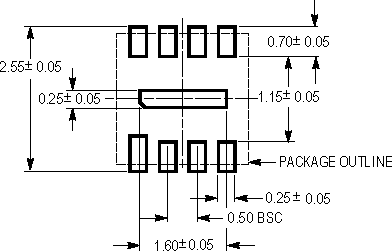
\includegraphics[width=0.5\textwidth]{LTC-Place.pdf}
	\caption{Рекомендуемое посадочное место.}%
	\label{fig:LTC-Place}
\end{figure}

Итоговый вид схемы можно увидеть на Рис~\ref{fig:LTC_Sch}.

\begin{figure}[!ht]
	\centering
	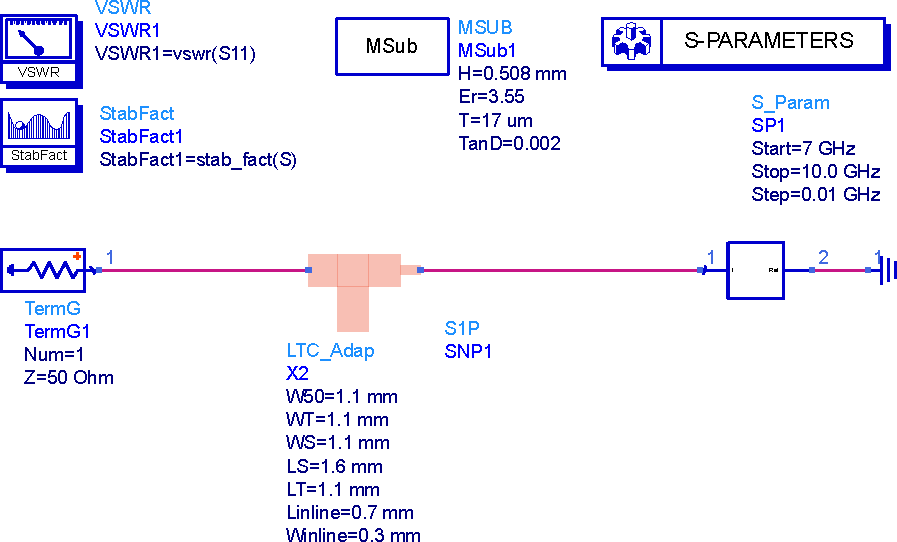
\includegraphics[width=\textwidth]{LTC_Sch.pdf}
	\caption{Схема включения детектора мощности.}%
	\label{fig:LTC_Sch}
\end{figure}

Результат согласования на Рис~\ref{fig:LTC-data}

\begin{figure}[H]
	\captionsetup{singlelinecheck=off, justification=centering}
	\centering
	\begin{subfigure}[b]{0.5\textwidth}
		\centering
		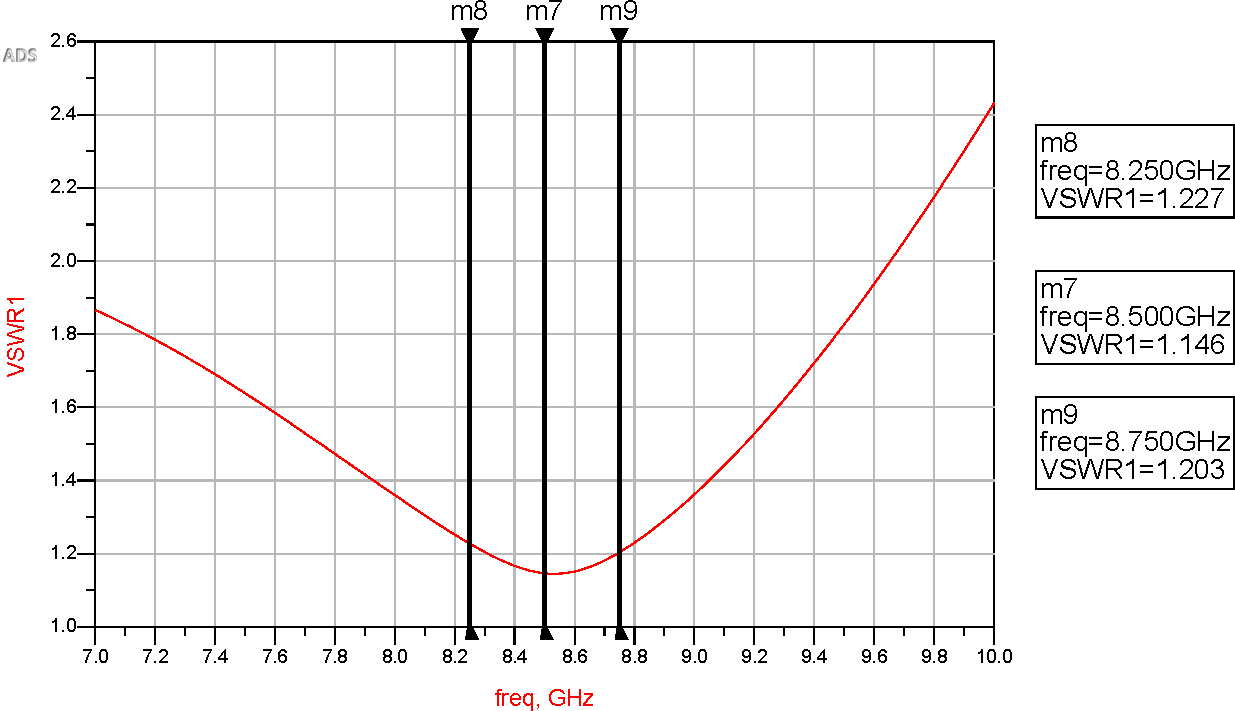
\includegraphics[width=\textwidth]{LTC_VSWR.pdf}
		\caption{}%
		\label{fig:LTC_VSWR}
	\end{subfigure}
	\hfill
	\begin{subfigure}[b]{0.45\textwidth}
		\centering
		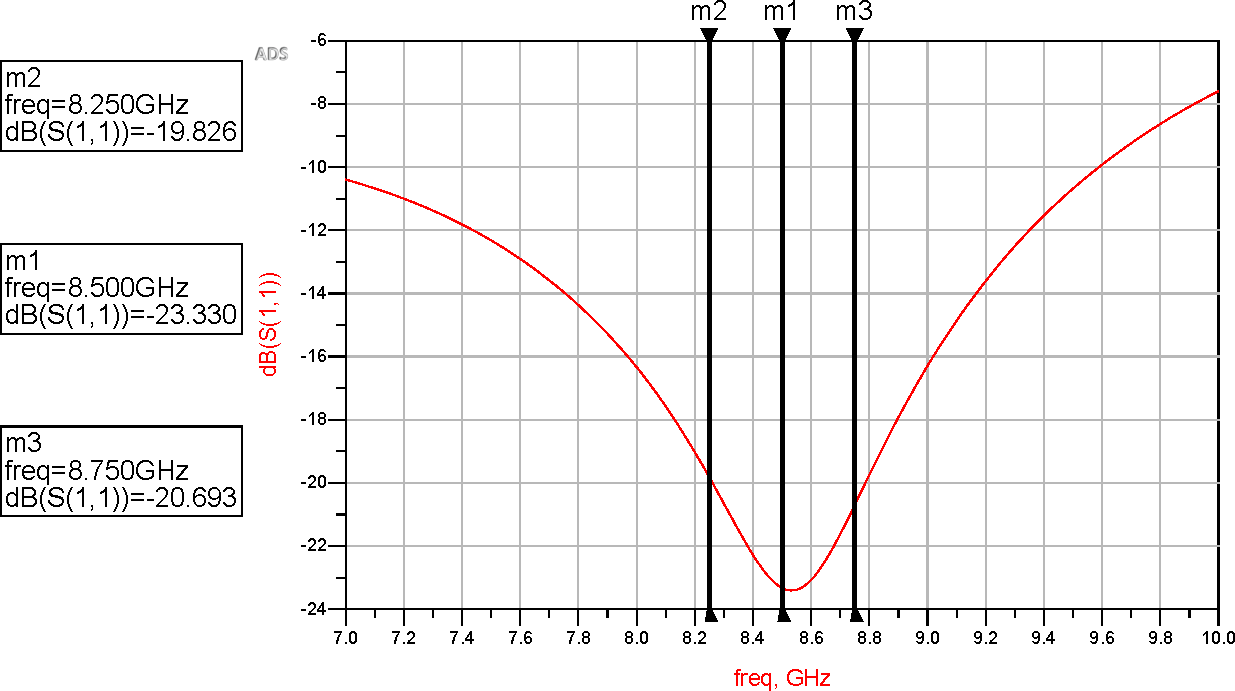
\includegraphics[width=\textwidth]{LTC_Response.pdf}
		\caption{}%
		\label{fig:LTC_Response}
	\end{subfigure}
	
	\caption{%
		Частотные характеристики согласованного детектора мощности:
		(а) КСВН;
		(б) АЧХ;
	}%
	\label{fig:LTC-data}
\end{figure}

\section{Проектирование фильтра}

Проектирование фильтра будем вести в среде Keysight Genesys.

\begin{figure}[H]
	\centering
	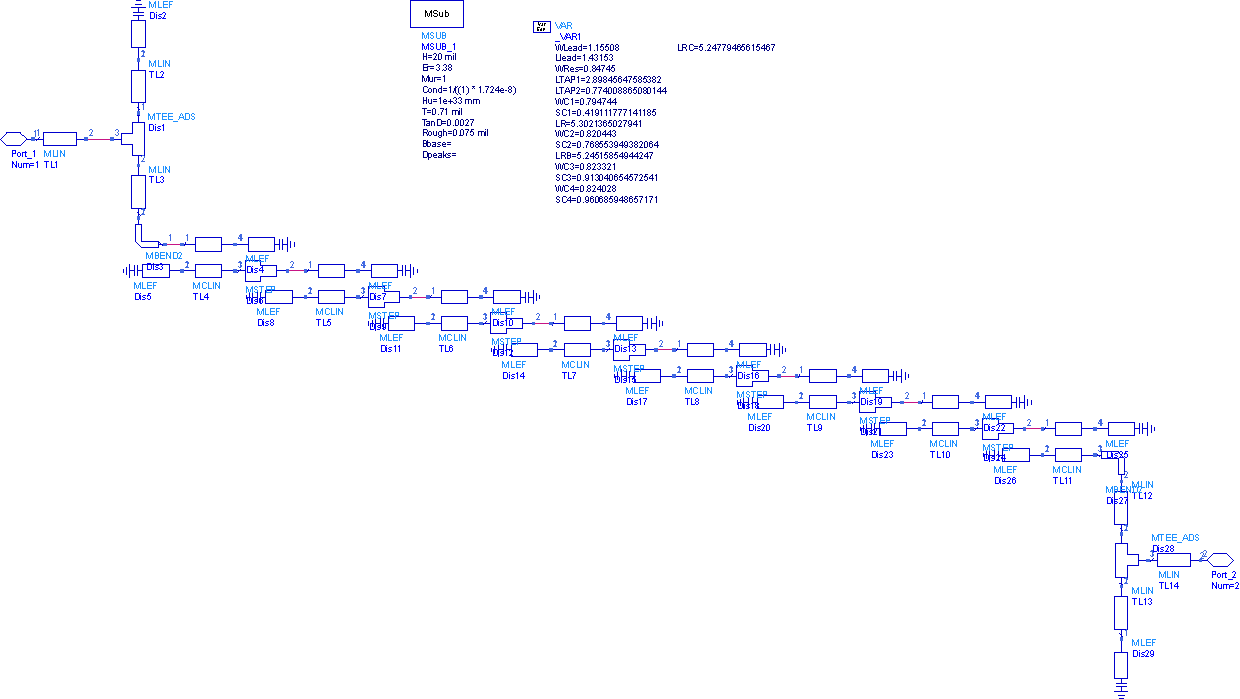
\includegraphics[width=0.9\textwidth]{FilterSch.pdf}
	\caption{Схема фильтра}%
	\label{fig:FilterSch}
\end{figure}

\begin{figure}[H]
	\centering
	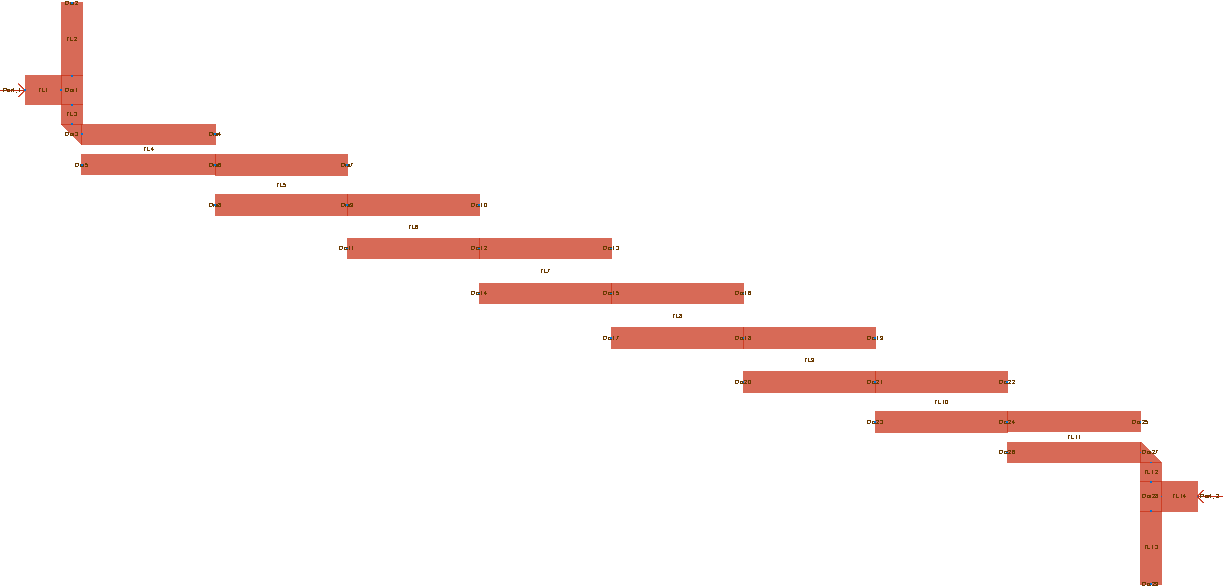
\includegraphics[width=\textwidth]{FilterLayout.pdf}
	\caption{Топология фильтра}%
	\label{fig:FilterLayout}
\end{figure}

\begin{figure}[H]
	\centering
	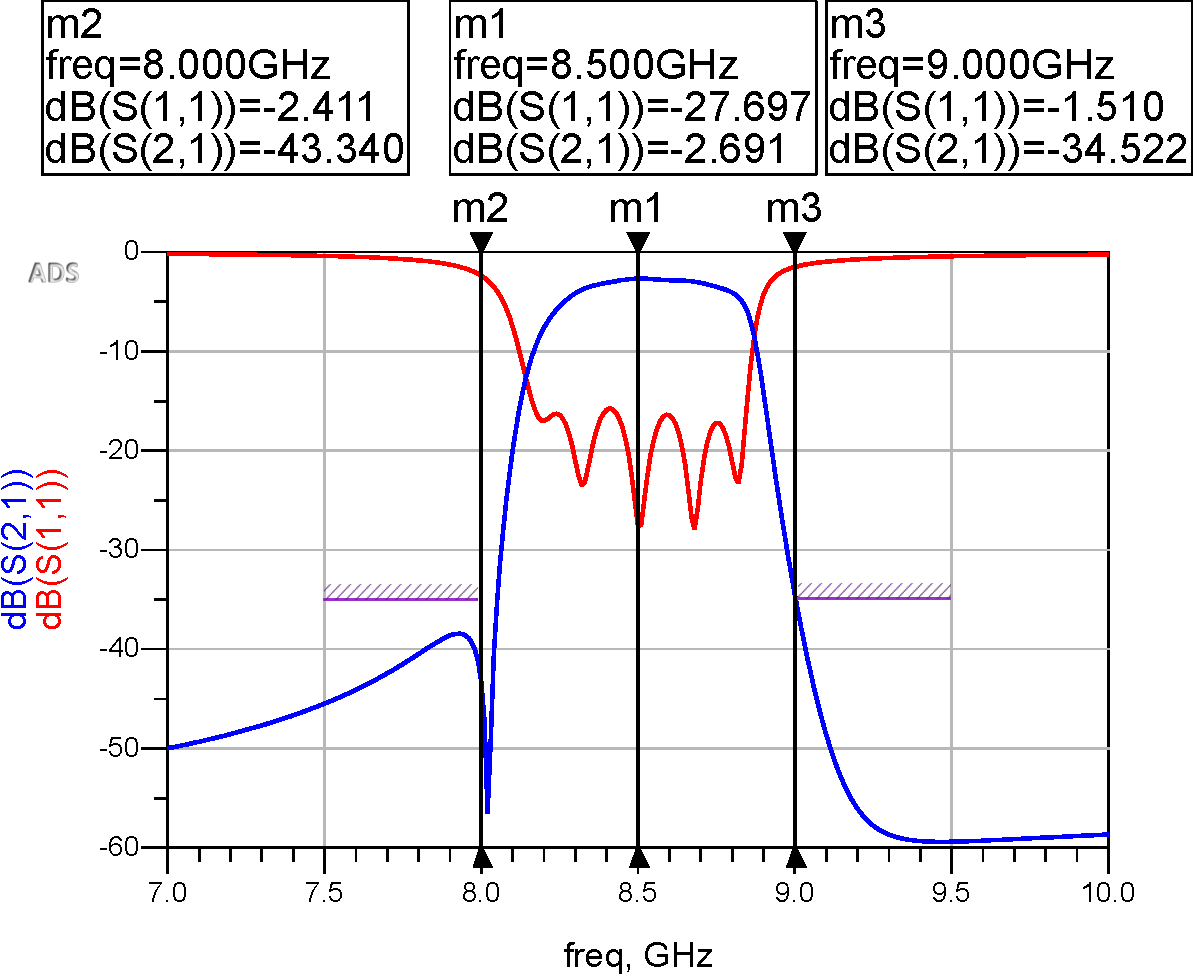
\includegraphics[width=0.8\textwidth]{FilterResponse.pdf}
	\caption{АЧХ фильтра}%
	\label{fig:FilterResponse}
\end{figure}

\section{Проектирование ответвителя}

Исходя из диапазона возможных входных значений, определяем ответвление в -40 дБ

\begin{figure}[H]
	\centering
	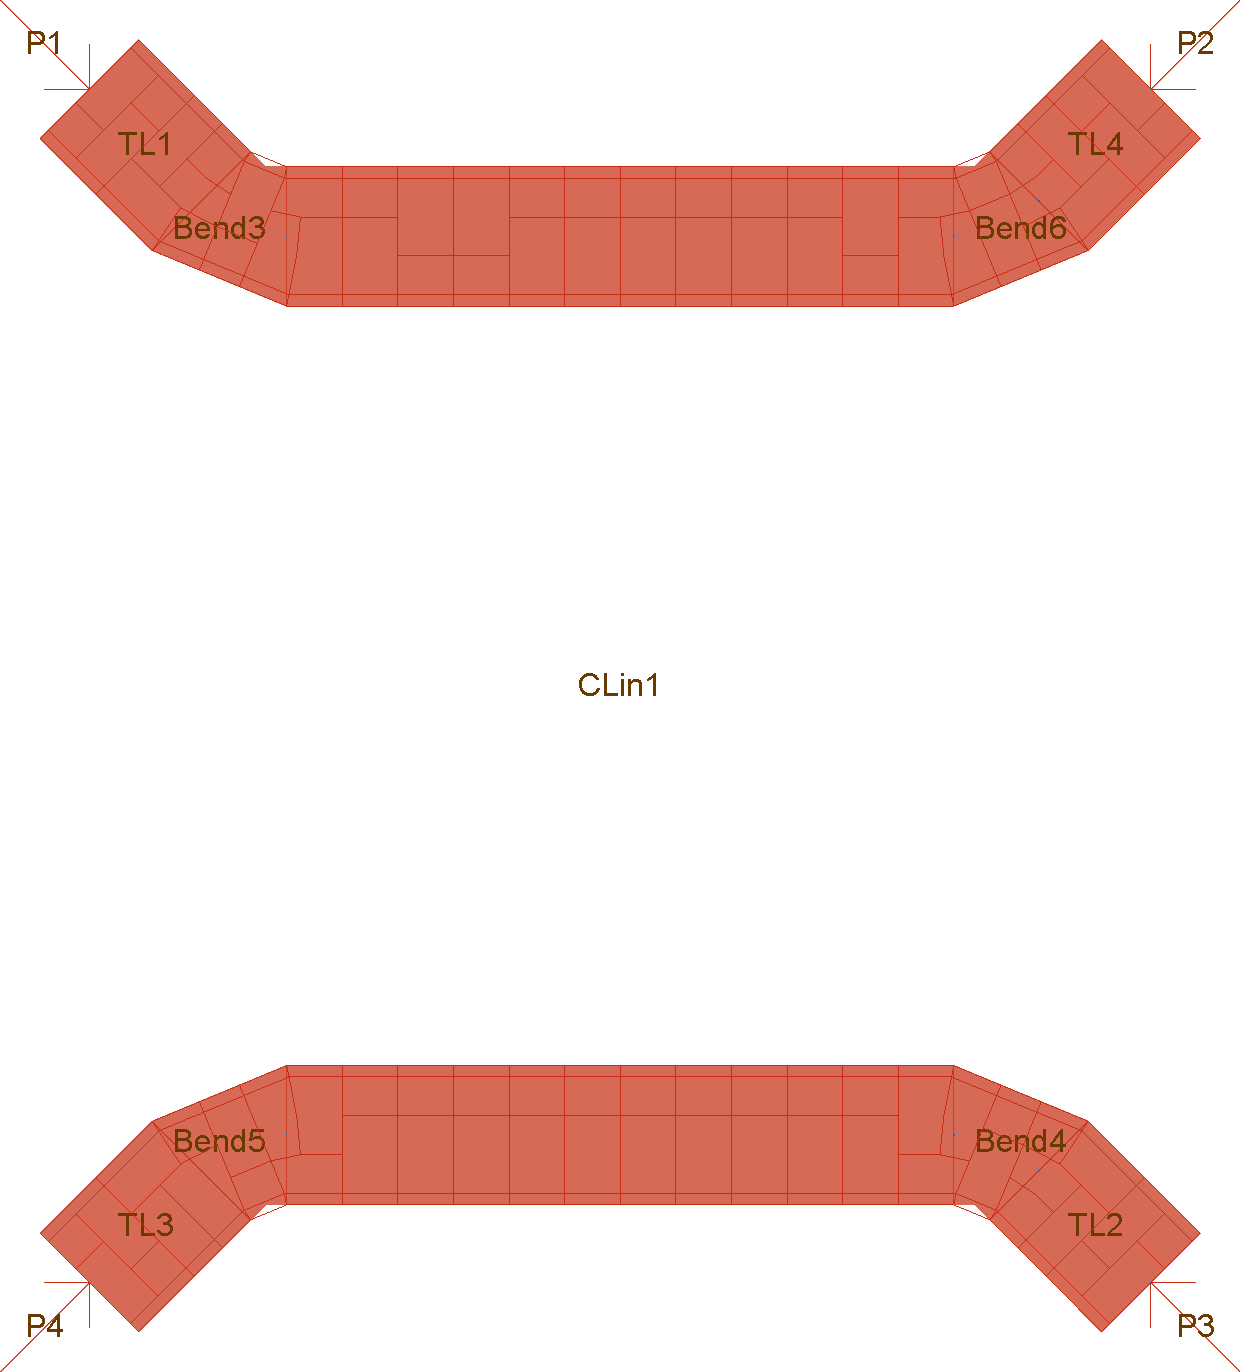
\includegraphics[width=0.4\textwidth]{CLC_Layout.pdf}
	\caption{Ответвитель на связных линиях}%
	\label{fig:CLC_Layout}
\end{figure}

\begin{figure}[H]
	\centering
	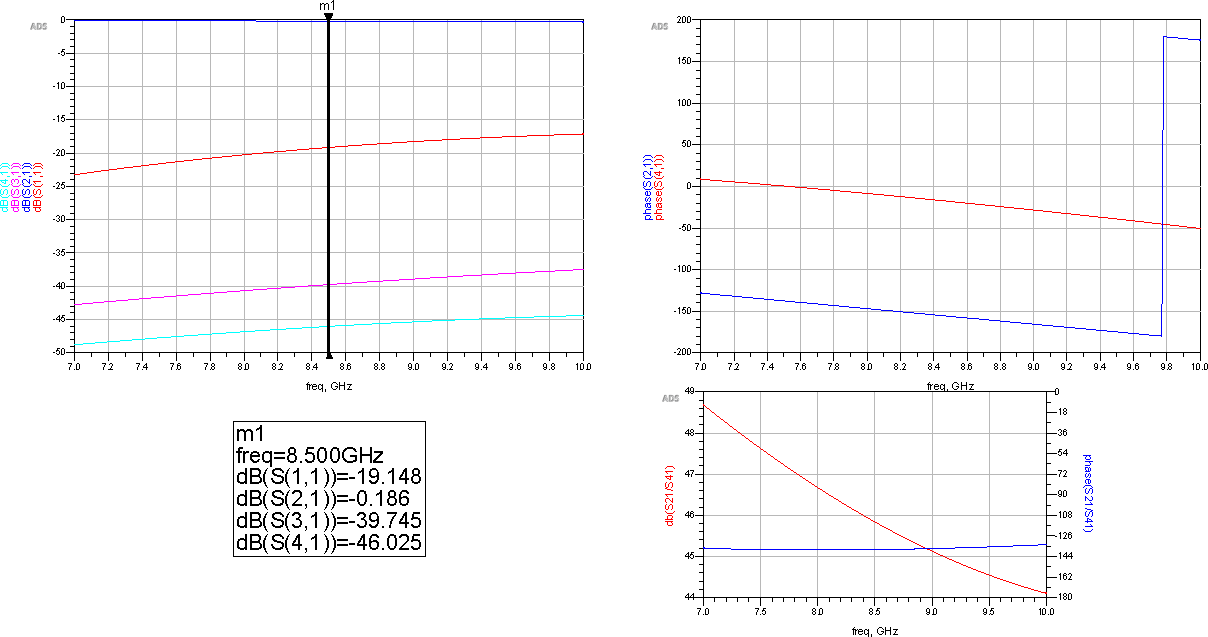
\includegraphics[width=\textwidth]{CLC_Response.pdf}
	\caption{Характеристика ответвителя}%
	\label{fig:CLC_Response}
\end{figure}